\documentclass[11pt]{article}

\usepackage[margin=1in]{geometry}
\usepackage{amsmath,amssymb}
\usepackage{booktabs}
\usepackage{graphicx}
\usepackage{float}
\usepackage{caption}
\usepackage{enumitem}
\usepackage{hyperref}
\usepackage{xcolor}
\usepackage{microtype}
\usepackage{array}

\hypersetup{
    colorlinks=true,
    linkcolor=blue,
    urlcolor=blue,
    citecolor=blue
}

\setlist[itemize]{leftmargin=1.5em}
\setlist[enumerate]{leftmargin=1.5em}
\setlength{\parindent}{0pt}
\setlength{\parskip}{0.7em}

\title{Weather Prediction-Market Trading Simulator\\\large Technical Project Report}
\author{}
\date{}

\begin{document}

\maketitle

\begin{abstract}
This project builds a Python simulator for trading a binary weather prediction market. The main contract asks whether Philadelphia will receive at least 0.50 inches of rain the following day. Historical and live forecast data are converted into event probabilities, calibrated with walk-forward validation, and then used as fair values for YES and NO contracts. The trading layer compares model fair value with executable bid and ask prices, applies an edge threshold, sizes positions with fractional Kelly sizing, enforces inventory and cash constraints, and settles contracts at either \$1 or \$0. The project also includes Monte Carlo simulation, a zero-edge control, a market-efficiency stress test, and Kelly-sizing sensitivity analysis. The calibrated probability model achieved an out-of-sample Brier score of 0.0877 versus 0.1007 for a base-rate benchmark, corresponding to 12.9\% Brier skill over the benchmark. Positive trading P\&L in the Monte Carlo section is conditional on the assumptions of the synthetic market and is not interpreted as evidence of real-world alpha.
\end{abstract}

\tableofcontents
\newpage

\section{Project Motivation}

Prediction markets convert uncertain future events into tradable contracts. A binary contract can be interpreted as a market-implied probability when the payoff is \$1 if the event occurs and \$0 otherwise. This makes weather events a useful setting for studying the connection between forecasting, probability calibration, market pricing, execution, and risk management.

The central question in this project is:

\begin{quote}
Will Philadelphia receive at least 0.50 inches of rain tomorrow?
\end{quote}

A YES contract pays \$1 if the event occurs and \$0 otherwise. A NO contract pays \$1 if the event does not occur and \$0 otherwise.

The goal is not just to predict rain. The project is designed to connect four separate problems:

\begin{enumerate}
    \item estimating the probability of the weather event,
    \item checking whether those probability estimates are well calibrated out of sample,
    \item translating probabilities into executable trading decisions, and
    \item testing whether the strategy behaves sensibly under different market assumptions.
\end{enumerate}

\section{Data}

The simulator uses Open-Meteo forecast and historical weather data for Philadelphia. The historical sample used in the current version contains 90 aligned forecast and realized-precipitation observations.

The event threshold is
\[
T = 0.50 \text{ inches}.
\]

Of the 90 observations, 11 were YES events and 79 were NO events, giving a historical base rate of
\[
\hat p_{\text{base}} = \frac{11}{90} \approx 0.1222.
\]

Forecast error is defined as
\[
e_i = y_i - f_i,
\]
where $y_i$ is realized precipitation and $f_i$ is the corresponding forecast. In the current sample, the mean forecast error is $-0.0656$ inches and the standard deviation is $0.4372$ inches.

The historical realized values are based on Open-Meteo historical/reanalysis data rather than an exchange-specific settlement feed. This is sufficient for a modeling project, but it is an important limitation when interpreting the results.

\section{Probability Model}

\subsection{Empirical forecast-error model}

The main probability model uses the empirical distribution of historical forecast errors rather than assuming a specific parametric distribution.

For a new precipitation forecast $f^*$, each historical forecast error is replayed as a possible realization:
\[
\tilde y_i = \max(0, f^* + e_i).
\]

The raw empirical probability of the event is then
\[
\hat p_{\text{raw}}
=
\frac{1}{n}
\sum_{i=1}^{n}
\mathbf{1}\{\tilde y_i \geq T\}.
\]

This approach keeps the historical error distribution, including its asymmetry and large misses, instead of forcing forecast errors into a Normal model. A Normal-error model was also tested during development, but the empirical model became the main model because it required fewer distributional assumptions.

\subsection{Probability calibration}

The raw empirical probabilities were too aggressive in parts of the probability range. To reduce overconfidence, I shrink the raw estimate toward the historical base rate:
\[
p_{\text{cal}}
=
(1-\lambda)\hat p_{\text{base}}
+
\lambda \hat p_{\text{raw}}.
\]

The parameter $\lambda$ controls how much weight is placed on the empirical forecast signal. At $\lambda=0$, the model uses only the historical base rate. At $\lambda=1$, the model uses the raw empirical estimate with no shrinkage.

Candidate values are tested on a grid from 0.0 to 1.0 in increments of 0.1. The current full-sample choice is
\[
\lambda = 0.50.
\]

\section{Walk-Forward Validation}

The probability model is evaluated using walk-forward validation. The first 45 observations form the initial training window. Day 46 is predicted using only days 1--45, day 47 is predicted using only days 1--46, and so on. This produces 45 genuinely out-of-sample predictions.

For each training window, the shrinkage parameter is selected using only data available inside that window. This prevents the held-out observation from influencing the calibration parameter.

The main evaluation metric is the Brier score:
\[
\text{Brier}
=
\frac{1}{N}
\sum_{i=1}^{N}(p_i-y_i)^2,
\]
where $p_i$ is the predicted probability and $y_i\in\{0,1\}$ is the event outcome. Lower values are better.

The out-of-sample results are shown in Table~\ref{tab:brier}.

\begin{table}[H]
\centering
\caption{Out-of-sample probability validation}
\label{tab:brier}
\begin{tabular}{lr}
\toprule
Model & Brier score \\
\midrule
Base-rate benchmark & 0.1007 \\
Raw empirical model & 0.1150 \\
Calibrated empirical model & 0.0877 \\
\bottomrule
\end{tabular}
\end{table}

Relative to the base-rate benchmark, the calibrated model has Brier skill
\[
1 - \frac{0.0877}{0.1007} \approx 12.9\%.
\]

The raw empirical model was worse than simply using the base rate. That result was useful because it showed that a model can look intuitively reasonable while still being poorly calibrated out of sample. Shrinkage improved the result enough to outperform the benchmark.

The average lambda selected across the walk-forward test was 0.482, close to the final full-history value of 0.50.

\begin{figure}[H]
\centering
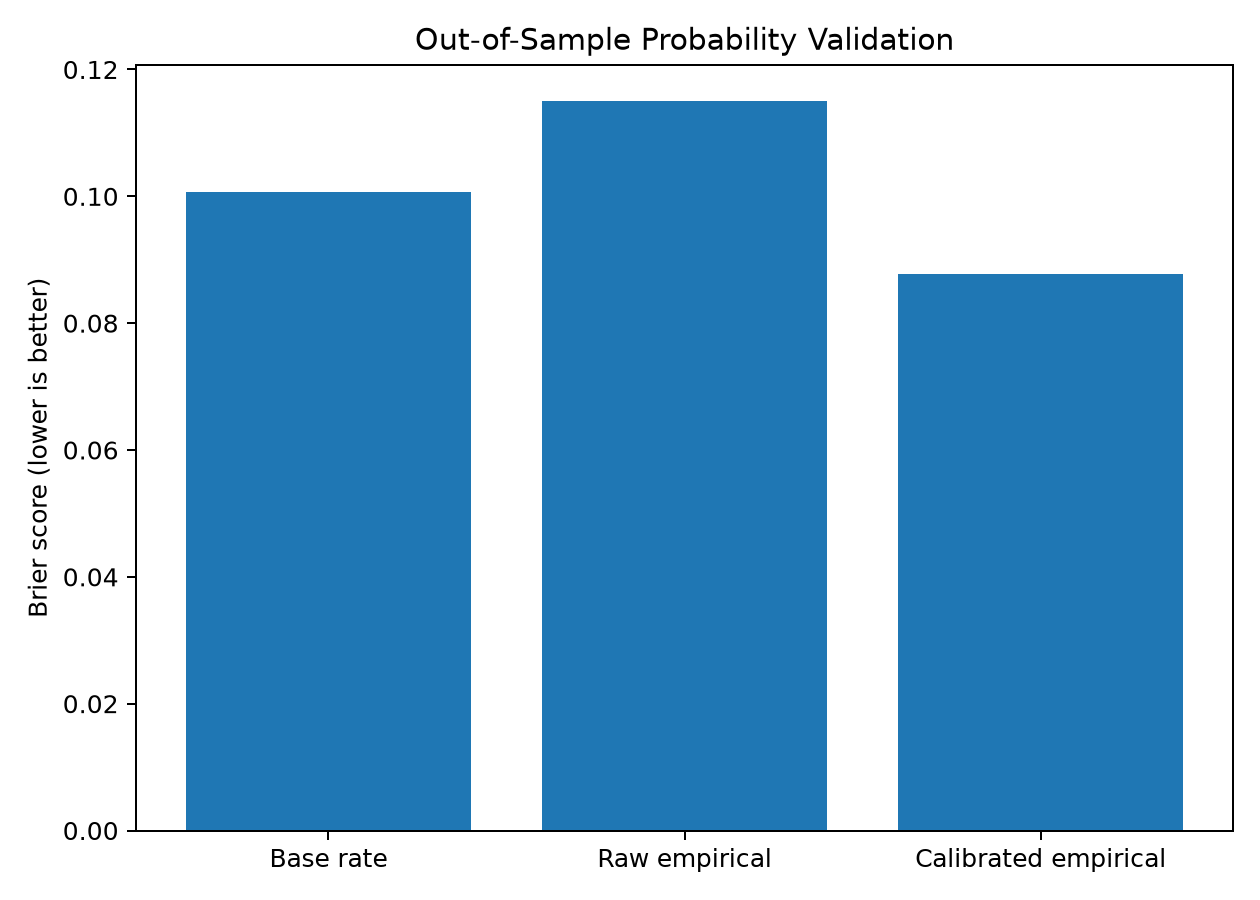
\includegraphics[width=0.88\linewidth]{results/brier_score_comparison.png}
\caption{Out-of-sample Brier score comparison. Lower is better.}
\label{fig:brier}
\end{figure}

\subsection{Calibration curve}

I also compare average predicted probability with observed event frequency. The current expected calibration error is 0.0825. The calibration curve is noisy because the walk-forward sample contains only 45 predictions and only 5 YES outcomes. High-probability bins in particular contain very few observations, so I treat this chart as a diagnostic rather than a precise estimate of long-run calibration.

\begin{figure}[H]
\centering
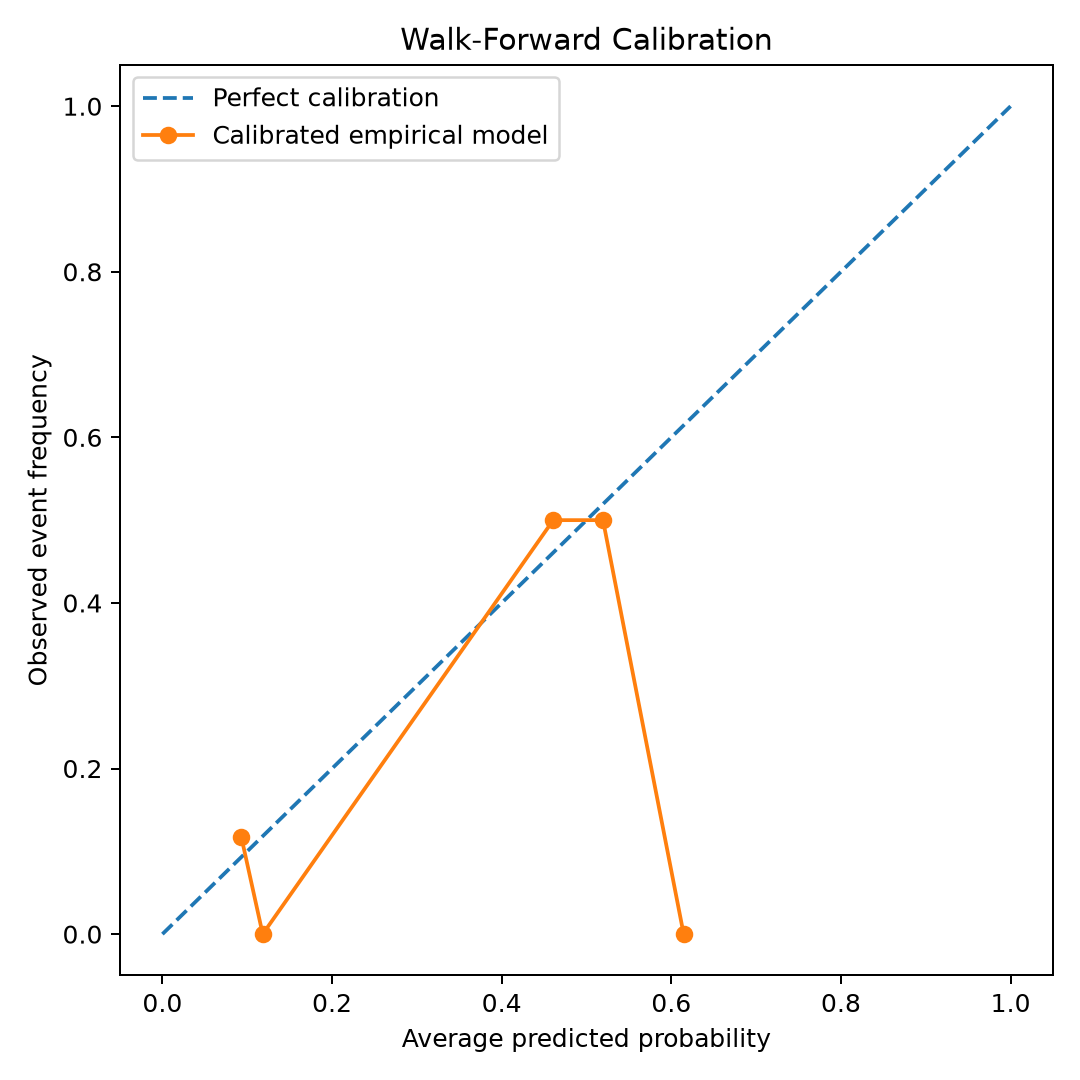
\includegraphics[width=0.78\linewidth]{results/calibration_curve.png}
\caption{Walk-forward calibration curve.}
\label{fig:calibration}
\end{figure}

\section{Sequential Forecast Updating}

The simulator also models the fact that weather forecasts can change during the day. A naive implementation would repeatedly treat each new forecast as independent evidence. That produced unrealistically large probability swings because intraday forecasts are strongly correlated.

The final version uses a dependence-aware odds-revision rule. Define the odds transform
\[
O(p)=\frac{p}{1-p}.
\]

Let $s_t$ be the calibrated probability implied by the current weather forecast and let $p_{t-1}$ be the previous posterior probability. The update has the form
\[
O(p_t)
=
O(p_{t-1})
\left(
\frac{O(s_t)}{O(s_{t-1})}
\right)^w,
\]
for later intraday revisions, where
\[
w=0.50.
\]

The first update is referenced to the historical prior rather than a previous intraday signal. Using $w<1$ discounts repeated information and prevents the model from becoming overconfident simply because similar forecasts arrive multiple times.

This is best viewed as a Bayesian-style, dependence-aware odds revision rather than a fully estimated conditional-likelihood model. A more rigorous version would require historical intraday forecast trajectories so that transition likelihoods could be estimated directly.

\section{Contract Valuation and Market Mechanics}

For a binary contract, the model probability becomes the fair value:
\[
FV_{\text{YES}} = p,
\qquad
FV_{\text{NO}} = 1-p.
\]

If the YES market is quoted with bid $b_Y$ and ask $a_Y$, the complementary NO market is
\[
b_N = 1-a_Y,
\qquad
a_N = 1-b_Y.
\]

The strategy uses executable prices rather than midpoints. Buying YES costs the YES ask and buying NO costs the NO ask. The corresponding model edges are
\[
\text{Edge}_{\text{YES}} = FV_{\text{YES}} - a_Y,
\]
\[
\text{Edge}_{\text{NO}} = FV_{\text{NO}} - a_N.
\]

The final strategy requires a minimum executable edge of 0.08 before entering a new position.

\section{Position Sizing and Risk Management}

\subsection{Fractional Kelly sizing}

For a binary contract with model probability $p$ and purchase price $c$, the full Kelly fraction of capital committed to a positive-edge long position is
\[
f^* = \frac{p-c}{1-c},
\]
provided $p>c$.

The strategy uses half Kelly:
\[
f = 0.50 f^*.
\]

Position size is also restricted by a maximum cash fraction and a hard position cap. The main settings are:

\begin{table}[H]
\centering
\caption{Main trading parameters}
\begin{tabular}{lr}
\toprule
Parameter & Value \\
\midrule
Minimum executable edge & 0.08 \\
Kelly fraction & 0.50 \\
Maximum cash fraction & 0.40 \\
Position cap & 50 contracts \\
Revision weight & 0.50 \\
Model-exit buffer & 0.02 \\
Baseline total spread & 0.02 \\
\bottomrule
\end{tabular}
\end{table}

The strategy does not hold YES and NO at the same time. If the model changes sides, the existing opposing position is reduced or closed before a new position is opened.

A position can also be closed before settlement if the executable bid moves sufficiently above the model's current fair value. Otherwise, positions can be held through binary settlement.

\subsection{Settlement and accounting}

At settlement, the correct side pays \$1 and the incorrect side pays \$0. Final P\&L is determined from the change in cash after all settlement payments. During the life of a position, marked inventory is valued at the executable bid rather than at the midpoint.

This distinction matters because entry cost determines realized and unrealized P\&L, while the current comparison between model fair value and bid/ask prices determines whether a new trade or model-based exit is attractive.

\section{Monte Carlo Trading Experiment}

The Monte Carlo section tests the trading logic across many synthetic weather and market paths. Each path contains a latent weather outcome, changing weather forecasts, changing market prices, bid/ask execution, position sizing, and settlement.

The baseline experiment is deliberately an informed-trader scenario: the strategy is assumed to have a faster or cleaner weather signal than the synthetic market. This is not meant to claim that real prediction markets systematically offer this advantage. It is a controlled environment for studying how the trading logic behaves when an information advantage exists.

The current baseline uses 1,000 Monte Carlo paths. Results are shown in Table~\ref{tab:mc}.

\begin{table}[H]
\centering
\caption{Baseline informed-trader Monte Carlo results}
\label{tab:mc}
\begin{tabular}{lr}
\toprule
Metric & Result \\
\midrule
Simulations & 1000 \\
Mean P\&L & \$6.12 \\
Median P\&L & \$9.07 \\
P\&L standard deviation & \$12.42 \\
Win rate & 72.8\% \\
Loss rate & 11.8\% \\
Flat rate & 15.4\% \\
5th percentile P\&L & -\$12.32 \\
95th percentile P\&L & \$19.09 \\
Worst P\&L & -\$40.51 \\
Best P\&L & \$43.29 \\
Average max drawdown & \$4.84 \\
95th percentile drawdown & \$18.36 \\
Average transactions & 1.50 \\
Position-cap hit rate & 66.9\% \\
\bottomrule
\end{tabular}
\end{table}

The median is above the mean because the distribution contains a left tail of relatively large losses. That tail is visible in Figure~\ref{fig:pnl} and is one reason the project reports the full distribution instead of focusing only on average P\&L.

\begin{figure}[H]
\centering
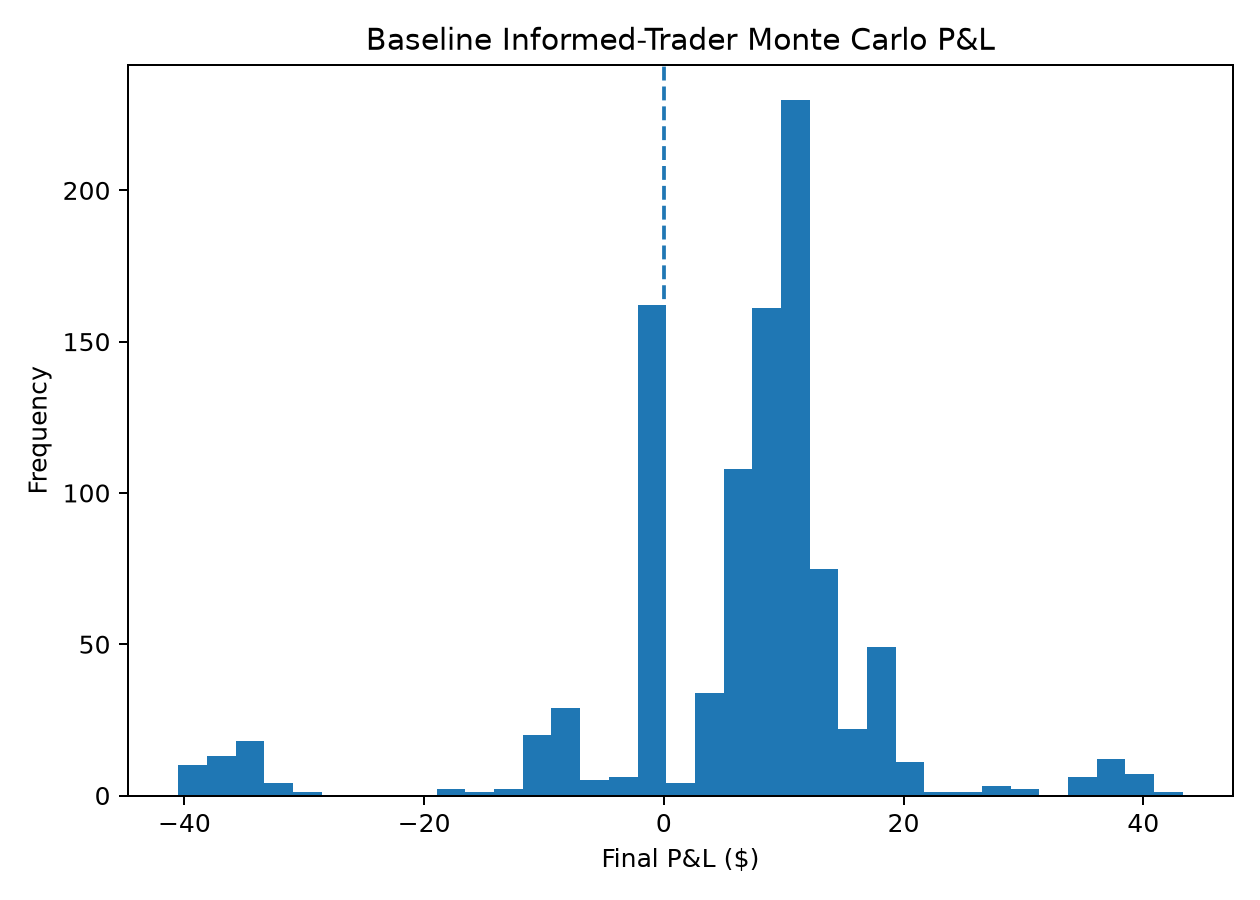
\includegraphics[width=0.90\linewidth]{results/pnl_distribution.png}
\caption{Distribution of final P\&L in the baseline informed-trader Monte Carlo experiment.}
\label{fig:pnl}
\end{figure}

\section{Zero-Edge Control}

A simulation can look profitable because of a bug in settlement, accounting, or price construction. To check for this, I run a zero-edge control in which the synthetic market is centered on the strategy's own fair value.

Under this control, the bid/ask spread leaves no executable positive edge. Across 1,000 paths, the strategy produced zero trades and zero P\&L:

\begin{table}[H]
\centering
\caption{Zero-edge control}
\begin{tabular}{lr}
\toprule
Metric & Result \\
\midrule
Mean P\&L & \$0.00 \\
Median P\&L & \$0.00 \\
P\&L standard deviation & \$0.00 \\
Win rate & 0.0\% \\
Loss rate & 0.0\% \\
Flat rate & 100.0\% \\
Average transactions & 0 \\
\bottomrule
\end{tabular}
\end{table}

This is an important sanity check because it confirms that positive simulated P\&L is not being mechanically created by the accounting system when no executable pricing edge exists.

\section{Market-Efficiency Stress Test}

The baseline Monte Carlo assumes an informational advantage. I therefore run a separate stress test that asks what happens as the market becomes more efficient relative to the trader.

In this test, the synthetic market midpoint moves toward the trader's current fair value according to
\[
M_t
=
M_{t-1}
+
\alpha(FV_t-M_{t-1})
+
\varepsilon_t,
\]
where $\alpha$ is market reaction speed and $\varepsilon_t$ is pricing noise.

Higher $\alpha$ means the market incorporates the trader's information more quickly. Lower noise means prices are cleaner. If the trader's advantage is really coming from temporary mispricing, simulated P\&L should decline as reaction speed increases and noise decreases.

That is what occurs in the final stress test. For example, with market noise standard deviation 0.02:

\begin{table}[H]
\centering
\caption{Mean P\&L as market reaction speed increases, noise SD = 0.02}
\begin{tabular}{rr}
\toprule
Reaction speed & Mean P\&L \\
\midrule
0.20 & \$3.34 \\
0.30 & \$2.95 \\
0.40 & \$2.60 \\
0.50 & \$2.10 \\
0.70 & \$0.75 \\
1.00 & \$0.00 \\
\bottomrule
\end{tabular}
\end{table}

When reaction speed reaches 1.00 and pricing noise is sufficiently low, the market essentially incorporates the model fair value immediately. The executable edge disappears and the strategy stops trading.

\begin{figure}[H]
\centering
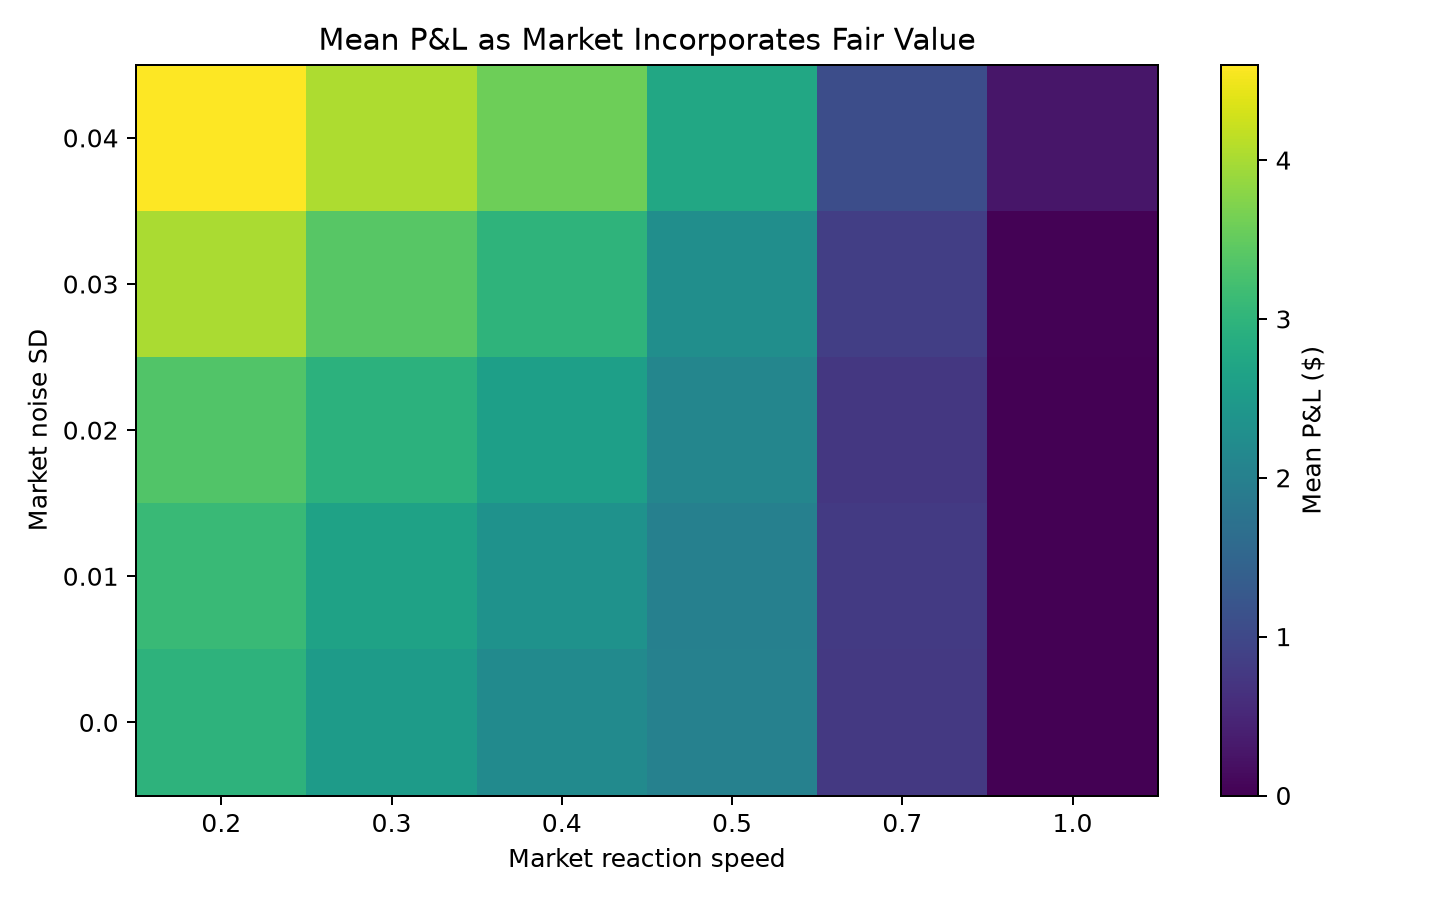
\includegraphics[width=0.92\linewidth]{results/market_efficiency_heatmap.png}
\caption{Mean P\&L across synthetic market reaction speeds and noise levels.}
\label{fig:efficiency}
\end{figure}

This experiment is useful because it gives the synthetic profitability an economic interpretation: the strategy makes money only when there is a temporary difference between the trader's estimate and the market price. As that difference disappears, so does the simulated edge.

\section{Kelly-Sizing Sensitivity}

I also test quarter Kelly, half Kelly, and three-quarter Kelly while keeping the rest of the baseline simulation fixed.

\begin{table}[H]
\centering
\caption{Kelly-sizing sensitivity}
\label{tab:kelly}
\begin{tabular}{rrrrrr}
\toprule
Kelly & Mean P\&L & P\&L SD & Win rate & Avg. drawdown & Cap hit \\
\midrule
0.25 & \$5.39 & \$11.72 & 72.9\% & \$3.74 & 33.9\% \\
0.50 & \$6.12 & \$12.42 & 72.8\% & \$4.84 & 66.9\% \\
0.75 & \$6.30 & \$12.66 & 72.6\% & \$5.28 & 71.2\% \\
\bottomrule
\end{tabular}
\end{table}

Moving from half Kelly to three-quarter Kelly increases average simulated P\&L by only \$0.18 while increasing volatility, drawdown, and position-cap usage. This is why the final baseline keeps half Kelly rather than choosing the most aggressive setting simply because it has the highest mean P\&L.

\begin{figure}[H]
\centering
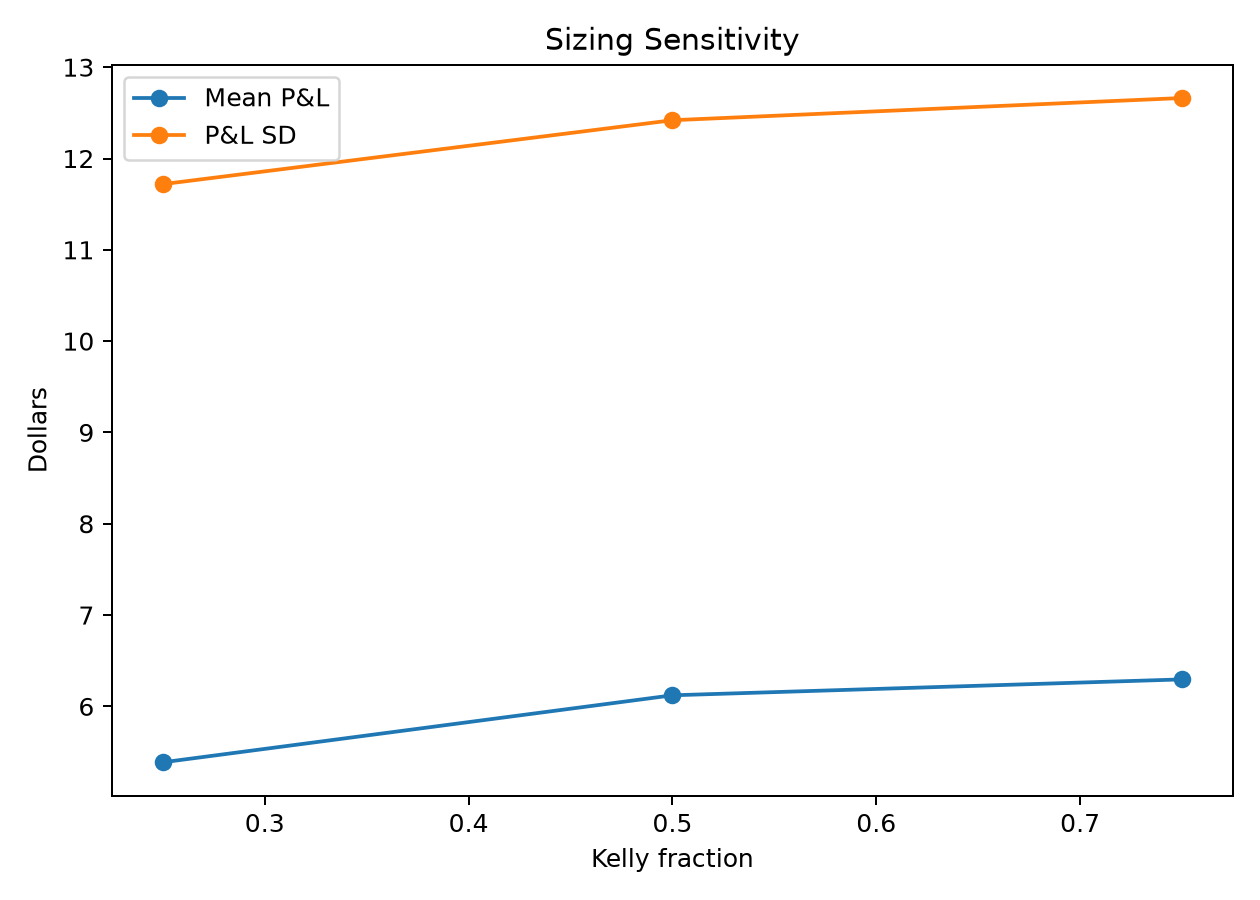
\includegraphics[width=0.88\linewidth]{results/kelly_sensitivity.png}
\caption{Mean P\&L and P\&L standard deviation across Kelly fractions.}
\label{fig:kelly}
\end{figure}

\section{What Changed During Development}

Several parts of the project changed after testing exposed weaknesses in earlier versions.

\subsection{Raw probabilities were not enough}

The initial empirical probability model looked reasonable, but its out-of-sample Brier score was worse than the base-rate benchmark. I added shrinkage and selected the shrinkage parameter using nested walk-forward validation. The calibrated model then achieved a lower Brier score than both the raw empirical model and the base-rate benchmark.

\subsection{Sequential updates were initially too aggressive}

An earlier update rule repeatedly treated intraday forecasts as independent evidence. Because weather forecast revisions are correlated, probabilities collapsed too quickly in some cases. The final odds-revision rule discounts later updates with a revision weight of 0.50.

\subsection{Forced end-of-day liquidation distorted the trading problem}

An earlier version forced the strategy to liquidate inventory at the final intraday quote. That mixed forecasting performance with an arbitrary liquidation rule. The final strategy allows positions to be held to binary settlement, while still permitting model-based exits before settlement.

\subsection{The first market-efficiency test had the wrong interpretation}

In an earlier synthetic stress test, increasing market reaction speed meant the market reacted faster to its own separate noisy signal. Faster reaction could therefore move price farther away from the trader's fair value and create more apparent edge. The final efficiency test instead defines efficiency as faster convergence toward the trader's current fair value. Under that definition, simulated edge correctly disappears as the market becomes fully efficient.

\section{Limitations}

The project has several important limitations.

\begin{itemize}
    \item The historical sample contains only 90 aligned observations and 11 YES events.
    \item The walk-forward test contains only 45 predictions and 5 YES events, so calibration estimates are noisy.
    \item Open-Meteo historical/reanalysis precipitation is not the same thing as an exchange's official settlement source.
    \item The synthetic market does not use historical prediction-market order-book data.
    \item Market reaction speed, pricing noise, forecast-error persistence, and spreads are modeling assumptions.
    \item The intraday odds-revision rule is dependence-aware but is not estimated from a full historical dataset of intraday forecast transitions.
    \item Monte Carlo profitability is conditional on an assumed information advantage and should not be interpreted as a real-world expected return.
\end{itemize}

These limitations are part of the reason I separate forecast validation from trading simulation. The out-of-sample Brier score tests the probability model against historical outcomes. The Monte Carlo P\&L tests strategy mechanics under explicit assumptions about how a market behaves. They answer different questions.

\section{Reproducibility and Project Structure}

The main Python script runs the data collection, probability model, validation, simulations, stress tests, and chart generation. Output CSV files and figures are written to the \texttt{results/} directory.

The main project structure is:

\begin{verbatim}
weather_predictions_market/
|-- main.py
|-- README.md
|-- report.tex
|-- report.pdf
|-- requirements.txt
|-- .gitignore
`-- results/
    |-- baseline_monte_carlo_pnl.csv
    |-- brier_score_comparison.png
    |-- calibration_curve.png
    |-- calibration_table.csv
    |-- kelly_sensitivity.csv
    |-- kelly_sensitivity.png
    |-- market_efficiency_heatmap.png
    |-- market_efficiency_stress_test.csv
    |-- pnl_distribution.png
    `-- walk_forward_predictions.csv
\end{verbatim}

The required Python packages are \texttt{requests}, \texttt{scipy}, and \texttt{matplotlib}. The project can be run with:

\begin{verbatim}
pip install -r requirements.txt
python main.py
\end{verbatim}

The LaTeX report can be compiled from the repository root with:

\begin{verbatim}
pdflatex report.tex
pdflatex report.tex
\end{verbatim}

or with \texttt{latexmk -pdf report.tex} if \texttt{latexmk} is installed.

\section{Conclusion}

This project started as a weather-based prediction-market simulator, but the most useful part of the work was separating the different sources of performance.

The probability model had to be judged on out-of-sample forecasting quality rather than on whether a simulated trade happened to make money. Walk-forward validation showed that the raw empirical model was overconfident, and shrinkage improved its Brier score from 0.1150 to 0.0877. The trading layer then introduced execution prices, edge thresholds, Kelly sizing, inventory constraints, and settlement. Finally, the zero-edge control and market-efficiency stress test checked whether simulated profits disappeared when the assumed informational advantage was removed.

The final result is therefore not a claim that the strategy would earn the reported Monte Carlo P\&L in a real prediction market. It is a framework for turning a probabilistic weather forecast into a trading decision, testing that decision under controlled market assumptions, and identifying which parts of the result come from forecasting quality, market inefficiency, and position sizing.

\begin{thebibliography}{9}

\bibitem{openmeteo}
Open-Meteo, ``Weather Forecast API and Historical Weather API.''
\url{https://open-meteo.com/}

\bibitem{brier}
G. W. Brier, ``Verification of Forecasts Expressed in Terms of Probability,'' \emph{Monthly Weather Review}, vol. 78, no. 1, pp. 1--3, 1950.

\bibitem{kelly}
J. L. Kelly Jr., ``A New Interpretation of Information Rate,'' \emph{Bell System Technical Journal}, vol. 35, no. 4, pp. 917--926, 1956.

\end{thebibliography}

\end{document}
